\centering
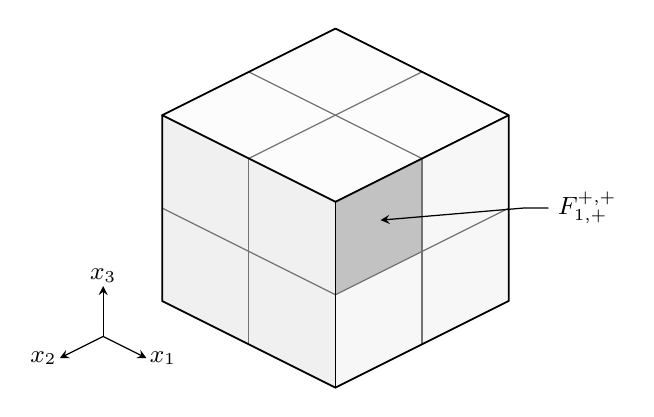
\begin{tikzpicture}[
  x={(1.10cm,-0.55cm)},
  y={(-1.10cm,-0.55cm)},
  z={(0cm,1.18cm)},
  font=\small,
  line join=round,
  line cap=round,
  >=stealth,
  qf edge/.style={black,line width=0.65pt},
  qf division/.style={black!55,line width=0.45pt}
]
  \fill[black!3] (1,-1,-1)--(1,1,-1)--(1,1,1)--(1,-1,1)--cycle;
  \fill[black!6] (-1,1,-1)--(1,1,-1)--(1,1,1)--(-1,1,1)--cycle;
  \fill[black!1] (-1,-1,1)--(1,-1,1)--(1,1,1)--(-1,1,1)--cycle;

  \fill[black!24] (1,0,0)--(1,1,0)--(1,1,1)--(1,0,1)--cycle;

  \draw[qf division] (1,0,-1)--(1,0,1);
  \draw[qf division] (1,-1,0)--(1,1,0);
  \draw[qf division] (0,1,-1)--(0,1,1);
  \draw[qf division] (-1,1,0)--(1,1,0);
  \draw[qf division] (0,-1,1)--(0,1,1);
  \draw[qf division] (-1,0,1)--(1,0,1);

  \draw[qf edge]
    (1,-1,-1)--(1,1,-1)--(-1,1,-1)--(-1,1,1)
    --(-1,-1,1)--(1,-1,1)--cycle;
  \draw[qf edge] (1,1,1)--(1,1,-1);
  \draw[qf edge] (1,1,1)--(-1,1,1);
  \draw[qf edge] (1,1,1)--(1,-1,1);

  \coordinate (qf representative) at (1,0.48,0.56);
  \begin{scope}[x=1cm,y=1cm]
    \node[anchor=west] (qf label) at (2.70,0.00) {$F_{1,+}^{+,+}$};
    \draw[->,line width=0.45pt]
      (qf label.west)--(2.38,0.00)--(qf representative);

    \coordinate (qf axes) at (-2.95,-1.63);
    \draw[->,line width=0.45pt]
      (qf axes)--(-2.40,-1.905) node[right,inner sep=1pt] {$x_1$};
    \draw[->,line width=0.45pt]
      (qf axes)--(-3.50,-1.905) node[left,inner sep=1pt] {$x_2$};
    \draw[->,line width=0.45pt]
      (qf axes)--(-2.95,-0.99) node[above,inner sep=1pt] {$x_3$};
  \end{scope}
\end{tikzpicture}
\caption{Quarter-faces of $\Lambda_b(u)$, shown schematically for $b>0$.
Each of the three visible faces is divided into four quarter-faces;
the three opposite faces are divided in the same way.
Thus $3$ normal axes $\times\,2$ normal signs $\times\,4$ transverse sign pairs
give $24$ quarter-faces. Boundary overlaps are permitted.
The shaded example $F_{1,+}^{+,+}$ has $x_1-u_1=b$ and
$0\le x_2-u_2,x_3-u_3\le b$.}
\label{prelim:quarterfaces-figure}
